% CAPÍTULO 3: DESCRIÇÃO DA SUA PROPOSTA OU CONTRIBUIÇÃO
%   ESSE É O CAPÍTULO MAIS IMPORTANTE DE SEU TRABALHO


%1. Elabore um parágrafo que introduz o capítulo: Este capítulo apresenta(descreva o objetivo do  capítulo...). É constituído de N seções a saber...
%2. Caso você tenha dúvida do nível de detalhamento da descrição, coloque-se no lugar do leitor!
%3. Elabore um parágrafo que conclui o capítulo e introduz o capítulo seguinte.


This chapter is about the proposed methodology of this master thesis experiment. The Figure \ref{fig:diag_metodologia} shows the phases and the tasks inside each phase. This chapter will explain each phase and task presented in the Figure \ref{fig:diag_metodologia}.

\begin{figure}[!htb]
    \centering
    \tikzstyle{every node}=[font=\large]
    
    \tikzstyle{task} = [rectangle, rounded corners, minimum width=4cm, minimum height=1.5cm,text centered, draw=black, fill=white!30, text width=3.5cm, font=\large]
    \tikzstyle{phase} = [rectangle, minimum width=4cm, minimum height=1.5cm,text centered, draw=black, fill=white!30, text width=5.0cm, font=\Large]
    \tikzstyle{--gray} = [ccmLGray, dashed, dash pattern=on 1cm off 1cm , rounded corners, line width = 2mm]
    \tikzstyle{--red} = [ccmRed, rounded corners, line width = 2mm]
    \tikzstyle{--blue} = [ccmDBlue, rounded corners, line width = 2mm]
    
    \tikzstyle{arrow_blue} = [ccmDBlue, rounded corners, line width = 2mm, ->]
    \tikzstyle{d--blue} = [ccmDBlue, dashed, dash pattern=on 1.0cm off 0.65cm, rounded corners, line width = 2mm]
    \tikzstyle{arrow_--_blue} = [ccmDBlue, dashed, dash pattern=on 1.0cm off 0.65cm, rounded corners, line width = 2mm, ->]
    \tikzstyle{arrow_red} = [ccmRed, rounded corners, line width = 2mm, ->]
    
    
    \resizebox{\linewidth}{!}{
    \begin{tikzpicture}[node distance=1cm]
        
        \node (interview) [phase] {Phase 1 – Context definition:};
        \node (interview_hospital) [task, below of = interview, yshift = -2cm] {1.1 Interview with environment specialists;};
        \node (interview_bvi) [task, below of = interview_hospital, yshift = -3.5cm] {1.2 Interview with BVI consultants.};
        
        \node (a1) [right of = interview, above of = interview, xshift = 2.0cm] {};
        \node (a2) [below of = a1, yshift = -11cm] {};
        \draw [--gray] (a1) to (a2);
        
        \node (scope) [phase] [phase, right of = interview, xshift = 5cm] {Phase 2 – Specification:};
        \node (virtual_environment) [task, below of = scope, yshift = -2cm] {2.1 Virtual environment specification;};
        \node (human_factors) [task, below of = virtual_environment, yshift = -2cm] {2.2 Assessment specification;};
        \node (guidance_methods) [task, below of = human_factors, yshift = -2cm] {2.3 Guidance specification.};
        
        \node (b1) [right of = scope, above of = scope, xshift = 2.0cm] {};
        \node (b2) [below of = b1, yshift = -11cm] {};
        \draw [--gray] (b1) to (b2);
        
        \node (development) [phase] [phase, right of = scope, xshift = 5cm] {Phase 3 – Development:};
        \node (ve_creation) [task, below of = development, yshift = -2cm] {3.1 Implementation of virtual environment;};
        \node (tools_definition) [task, below of = ve_creation, yshift = -2cm] {3.2 Proposal of assessment techniques and tools;};
        \node (guidance_development) [task, below of = tools_definition, yshift = -2cm] {3.3 Development of guidance devices.};
        
        \node (c1) [right of = development, above of = development, xshift = 2.0cm] {};
        \node (c2) [below of = c1, yshift = -11cm] {};
        \draw [--gray] (c1) to (c2);
        
        \node (tryouts) [phase] [phase, right of = development, xshift = 5cm] {Phase 4 – Preliminary evaluation:};
        \node (tryouts_task) [task, below of = tryouts, yshift = -5.0cm] {4.1 Try-outs.};
        
        \node (d1) [right of = tryouts, above of = tryouts, xshift = 2.0cm] {};
        \node (d2) [below of = d1, yshift = -11cm] {};
        \draw [--gray] (d1) to (d2);
        
        \node (experiment) [phase] [phase, right of = tryouts, xshift = 5cm] {Phase 5 – Systematic evaluation:};
        \node (experiment_task) [task, below of = experiment, yshift = -5.0cm] {5.1 Controlled experiments.};
    
        \draw[arrow_blue] (interview_hospital.east) to (virtual_environment.west);
        \draw[arrow_blue] (interview_bvi.east) to ++(1.0,0) to ++(0,4.5) to (virtual_environment.west);
        \draw[arrow_blue] (interview_bvi.east) to ++(1.0,0) to ++(0,1.5) to (human_factors.west);
        \draw[arrow_blue] (interview_bvi.east) to ++(1.0,0) to ++(0,-1.5) to (guidance_methods.west);  
        
        \draw[arrow_blue] (virtual_environment.east) to (ve_creation.west);
        \draw[arrow_blue] (human_factors.east) to (tools_definition.west);
        \draw[arrow_blue] (guidance_methods.east) to (guidance_development.west);
        
        \draw[arrow_blue] (ve_creation.east) to ++(1.0,0) to ++(0,-3.0) to (tryouts_task.west);
        \draw[arrow_blue] (tools_definition.east) to ++(1.0,0) to  (tryouts_task.west);
        \draw[arrow_blue] (guidance_development.east) to ++(1.0,0) to ++(0,3.0) to (tryouts_task.west);
        
        \draw[arrow_blue] (tryouts_task.east) to (experiment_task.west);
        \draw[--red] (tryouts_task.north) to (tryouts.south);
        \draw[--red] [opacity=0.2] (tryouts.south) to (tryouts.center) to (tryouts.west);
        \draw[arrow_red] (tryouts.west) to (development.east);

        \draw[d--blue] (experiment_task.north) to (experiment.south);
        \draw[d--blue] [opacity=0.2] (experiment.south) to (experiment.center) to (experiment.north);
        \draw[arrow_--_blue] (experiment.north) to ++(0,1.0) to ++(-18.0,0.0) to (scope.north);
        
    \end{tikzpicture}
    }
    \caption{Method's diagram}
    \label{fig:diag_metodologia}
\end{figure}


\section{Interviews' phase}
\label{sec:interviews_phase}
    The first phase of this project was the Interviews' phase. In this phase, the researchers' main goal was to gather information, especially those related to the COVID-19 pandemic, about the main procedures that happen inside a hospital and about the daily life of BVI people.

    \subsection{Interview with the hospital}
    
        To understand the procedures that hospitals and medical clinics followed during their day-to-day activities and the COVID-19 pandemic, two hospitals were interviewed. The interview was aimed to find out how a new patient does check-in and the following steps until he/she gets in the proper medic's office.
        
        At the project's start, the scenario was supposed to be a reception inside a hospital, but, because of the physical space needed to simulate that virtual environment, the scenario changed throughout the project several times.

    \subsection{Interview with the BVI consultants}
    
        One of the motivations of this master thesis is that the current BVI guidance products are not effective enough and one of the likely reasons is that the BVI users were not consulted during the product development process.
    
        With that thought in mind, BVI users were consulted to design a virtual environment that would be familiar with their reality. Two users with different visual impairments were interviewed, one person that became blind at 13 years old, and another with Usher's disease. These were critical to understanding how they perceive a medical clinic as they walk in and how they interact with the environment and these notes were used in the next phase.

\section{Experiment idealization's phase}
\label{sec:idealization_phase}
    At this phase, the proceedings and the interview notes are used to make key decisions about the virtual environment used in the experiment, which human factors are going to be assessed and which guidance methods are going to be used
    

    \subsection{Experiment's virtual world definition}
        As said before, the original idea was to use a hospital reception as a model for the virtual environment for the experiment, however, the physical space needed to fit the hospital was too big. So instead of a whole hospital reception, it was decided to use it as a medical clinic reception but still with the same proceedings.

    \subsection{Assessed human factors definition}
	To reach the experiment's objective, a set of human factors had to be chosen. The objectives \ref{itm:obj_second} and \ref{itm:obj_third} could be reached if the assessed human factor represented the user's workload and the developed mental map. Both these could be evaluated using:

        \begin{itemize}
            \item Mental workload
            \item Situation awareness
        \end{itemize}
        
        The details about each method are explained in the sections \ref{sec:mental_workload} and \ref{sec:situation_awareness}.

    \subsection{Guidance methods definition}
        The variety of BVI users is wide, as is the variety of assistive products. All of these products must communicate with the users and they use sound, vibration or both to transmit information. With this thought in mind, it was decided that it would be used at least two methods: one that relies only on audio and another that transmits only vibration. Of course, the interaction between those two methods would be also evaluated. This interaction became the third method.
        
        Another interesting property that could be evaluated in those products is the effect of information being transmitted with and without the user's command. This evaluation split the vibration method into two: one that worked \textit{without} the user's command and another that worked \textit{with} the user's command.
        
        At the end, the following methods were chosen to be analysed:
        
        \begin{itemize}
            \item A usual guidance method;
            \item Audio guidance;
            \item Vibration guidance without command;
            \item Vibration guidance with command;
            \item Mixture of audio and vibration.
        \end{itemize}
    
\section{Development and creation's phase}
\label{sec:creation_phase}
    
    With the decision of the previous phase it is possible to start the development of the virtual environment, the guidance methods and the tools for the assessment of the human factors.

    \subsection{Virtual world creation}
        The virtual reality application was made using the software Unity3D, which is a famous tool for virtual reality applications and game development. It has some built-in tools but is also possible to customize functions for more specific use \cite{wang2010new}. The virtual environments, or scenes (as it is called inside the Unity3D), were made with the dimensions to fit in the CCM entry hall, which has a flat area of 8x4m. Inside the environment, there was some typical furniture or devices found in hospital reception, a reception desk and a waiting area, composed of 2-3 chairs. The participant had \ref{itm:n_tasks} tasks at the scene and they are displayed at Figure \ref{fig:task_diagram}. More details ahead at Chapter \ref{ch:cenario}.
        
        \begin{enumerate}
            \item Clean the hands at the sanitizer totem (COVID-19 procedures);
            \item Go to the reception desk to receive a queue number;
            \item Go to the waiting area and wait for the number calling;
            \item Leave the room when called \label{itm:n_tasks}
        \end{enumerate}
        
        \begin{figure}[!htb]
    \centering
    \tikzstyle{every node}=[font=\large]
    
    \tikzstyle{task} = [rectangle, rounded corners, minimum width=4cm, minimum height=1.5cm,text centered, draw=black, fill=white!30, text width=3.5cm, font=\large]
    \tikzstyle{--gray} = [ccmGray, dashed, dash pattern=on 1cm off 1cm , rounded corners, line width = 2mm]
    \tikzstyle{--red} = [ccmRed, rounded corners, line width = 2mm]
    \tikzstyle{entryLine} = [ccmDBlue, rounded corners, line width = 2mm]
    \tikzstyle{arrow} = [ccmRed, rounded corners, line width = 1mm, ->]
    \tikzstyle{arrowX} = [line width = 2mm]
    
    \begin{tikzpicture}[node distance=1cm]
        
        \node (entryA) {};
        \node (exit) [below of = entryA, xshift = 0.5cm] {Exit};
        \node (entryB) [right of = entryA, xshift = 1.5cm] {};
        \node (entry) [below of = entryB, xshift = -0.5cm] {Entry};
        \draw[entryLine] (entryA) to (entryB);
        
        \node (totem) [right of = entryB, above of = entryB, draw, rectangle, minimum width=1cm, minimum height=1cm, draw=black, fill=white!30] {};
        \node (totemTexto) [below of = totem, yshift = 0.3cm, font = \small] {Sanitizer totem};
        
        \node (desk) [above of = entryB, yshift = 5.0cm, draw, rectangle, minimum width=3cm, minimum height=1.5cm, draw=black, fill=white!30, font = \small] {Reception};
        \node (nurse) [above of = desk, yshift = 0.6cm] {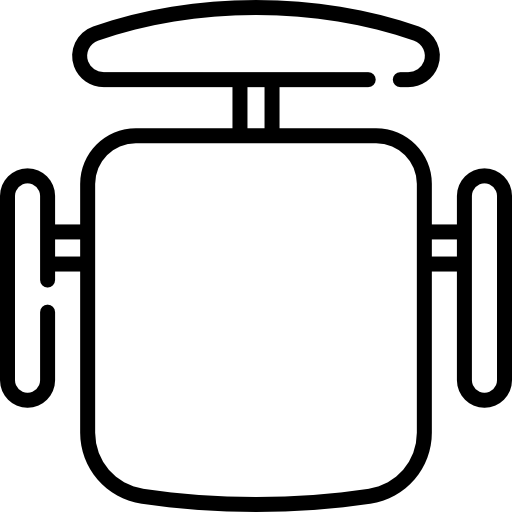
\includegraphics[scale = 0.09]{Metodologia/enfermeira.png}};
        \node (visitor) [below of = desk, yshift = -0.6cm] {
\includegraphics[angle=180, origin=c, scale = 0.09]{Metodologia/visita.png}};
        
        \node (waiting1) [left of = desk, xshift = -5.0cm] {
\includegraphics[angle=90, origin=c, scale = 0.09]{Metodologia/visita.png}};
        \node (waiting2) [below of = waiting1, yshift = -0.3cm] {
\includegraphics[angle=90, origin=c, scale = 0.09]{Metodologia/visita(x).png}};
        \node (waiting3) [below of = waiting2, yshift = -0.3cm] {
\includegraphics[angle=90, origin=c, scale = 0.09]{Metodologia/visita.png}};
        \node (waitingTexto) [left of = waiting2, rotate = 90, font = \small] {Waiting area};
        
        
        \draw (-5,0) rectangle(5cm,8.5cm);
        
        \draw[arrow] (entry) to ++(0,2.0) to (totem.west);
        \draw[arrow] (totem.north) to ++(0,0.5) to ++(-1.0,0) to (visitor.south);
        \draw[arrow] (visitor.west) to ++ (-3.0,0) to ++(0,-1.0cm) to (waiting3.east);
        \draw[arrow] (waiting3.south) to ++(0,-1.0) to ++(4.0,0) to (exit);  
        
    \end{tikzpicture}
    \caption{Scheduled task of the experiment and their order.}
    \label{fig:task_diagram}
\end{figure}

        
        The goal of these tasks is to engage the user to navigate through the room and see if it can draw a mental map of the scene as well as use the information about the obstacles to avoid them when needed. Besides these main components, there were some minor distractions that are common to hear at a clinical, such as telephone ringing, keyboard typing, people taking and others. These were put to increase the immersion and to be a distraction as well, otherwise, it wouldn't simulate the reality of these scenarios.
    
    \subsection{Tools and methods definition}
        There were three types of human factors assessment tools that were applied in the experiment:
        \begin{itemize}
            \item Task performance; \\  Measured using the time and the number of contacts between the user and the furniture throughout the experiment.
            \item Physiological measures; \\ Measured using an ECG sensor, a GSR sensor and a temperature sensor.
            \item Subjective measures. \\ Measured using a NASA-TLX, a SAGAT Adapted questionnaire and a guidance method evaluation questionnaire.
        \end{itemize}
        The details about each method are explained in the sections \ref{subsec:task_performance}, \ref{subsec:physiological_measures} and \ref{subsec:subjective_measures}.
        
    \subsection{Guidance methods development}
        As said in the last section, three different guidance methods were established to be used in the experiment besides the White Cane, a haptic belt and a virtual cane.
        \begin{itemize}
            \item A audio guidance method; \\ The audio-only guidance method will be straight and simple. In the course of the experiment the participant could give two different voice commands:
            \begin{itemize}
                \item  "What is around me?"; \\ The answer to this command was a quick description of the closest furniture around the user.
                \item  "Where is (something)?". \\ The answer of this command was the direction and distance of something asked by the user.
            \end{itemize}
            Each command was answered by a member of the experiment team accordingly.
            
            \item The haptic belt; \\
            That is a belt that had appended 8 vibration devices that vibrate accordingly to the direction and distance of the closest object around the user. More information on the Haptic Belt ahead at Chapter \ref{ch:cinto}.
            
            \item The virtual cane. \\ 
            This was based on the white cane mechanics, that the user "points" the cane to check near obstacles in the direction of the cane. The virtual cane has a similar function, but instead of connecting the user to the object through the cane, it vibrates when it detects an obstacle in the direction pointed by the user. A VR hand-control was used as canes and the user point it to where he/she wanted. The algorithm used on the Virtual Cane is in the Appendix \ref{ap:virtual_apend}
        \end{itemize}
    

\section{Tryouts and tests' phase}
\label{sec:tests_phase}
        
        At this phase, a few tests were performed to evaluate if the experiment was going as planned and to avoid any unfortunate events or errors during the real experiment. It was expected that changes could be needed to be made before the real experiment and there were a few. It was at this phase that the final dimension of the virtual environment and the physical space were defined.

\section{Experiment}
\label{sec:experiment}
        
        As the proper section name says, this phase is where the proper experiment was made.

After all these phases were completed, the next step was to analyze all the data and elaborate their conclusions. Instead of going to the results and discussions, the next Chapters \ref{ch:cenario} and \ref{ch:cinto} will deepen in the virtual environment development and the haptic belt development in these order. The Figure \ref{fig:ve_re} shows a comparison between the virtual environment created in Unity3D and the real environment assembled in the CCM's entry hall.

%\begin{figure}[!htb]
    \centering
    \tikzstyle{every node}=[font=\large]
    
    \tikzstyle{task} = [rectangle, rounded corners, minimum width=4cm, minimum height=1.5cm,text centered, draw=black, fill=white!30, text width=3.5cm, font=\large]
    \tikzstyle{phase} = [rectangle, minimum width=4cm, minimum height=1.5cm,text centered, draw=black, fill=white!30, text width=3.5cm, font=\Large]
    \tikzstyle{--} = [black, line width = 2mm]
    \tikzstyle{--red} = [ccmRed, rounded corners, line width = 2mm]
    \tikzstyle{arrow_blue} = [ccmDBlue, rounded corners, line width = 2mm, ->]
    \tikzstyle{arrow_red} = [ccmRed, rounded corners, line width = 2mm, ->]
    
    
    \setlength{\fboxsep}{0pt}%
    \setlength{\fboxrule}{1mm}

    \resizebox{\linewidth}{!}{
    \begin{tikzpicture}[node distance=1cm]
        
        \node (image1) [] {\fbox{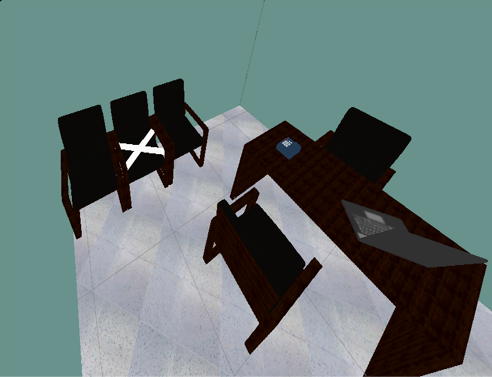
\includegraphics[width = 0.5\linewidth]{Metodologia/VE.png}}};
        \node (image2) [right of = image1, xshift = 7.15cm] {\fbox{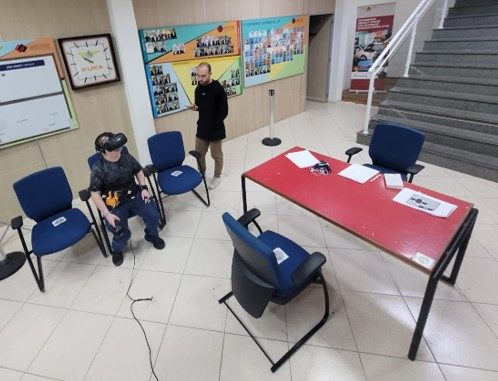
\includegraphics[width = 0.5\linewidth]{Metodologia/RE.jpg}}};

        \node (image3) [below of = image1, yshift = -10cm] {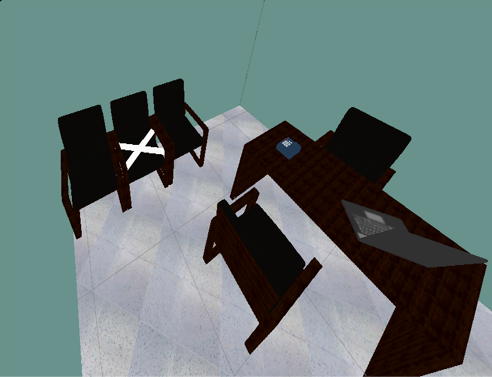
\includegraphics[width = 0.5\linewidth]{Metodologia/VE.png}};
        \node (image4) [right of = image3, xshift = 7.15cm] {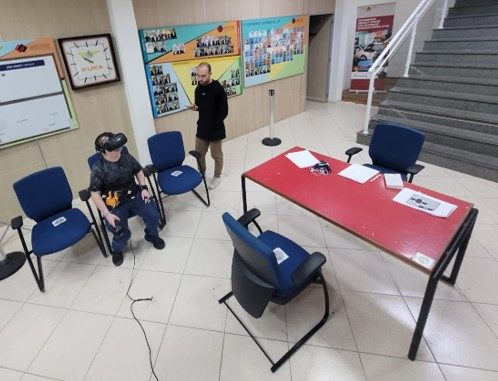
\includegraphics[width = 0.5\linewidth]{Metodologia/RE.jpg}};

        %\node (ponto1) [above of = image1, yshift = 2.5cm, left of = image1, xshift = -3cm] {};
        %\node (ponto2) [above of = image1, yshift = 2.5cm, right of = image1, xshift = 3cm]{};
    
        %\draw[--] (ponto1.west) -- (ponto2.east);
        
    \end{tikzpicture}
    }
    \caption{Virtual and Real environment comparisson}
    \label{fig:ve_re}
\end{figure}

\begin{figure}[!htb]
    \centering
    \begin{subfigure}[b]{0.49\textwidth}
        \centering
        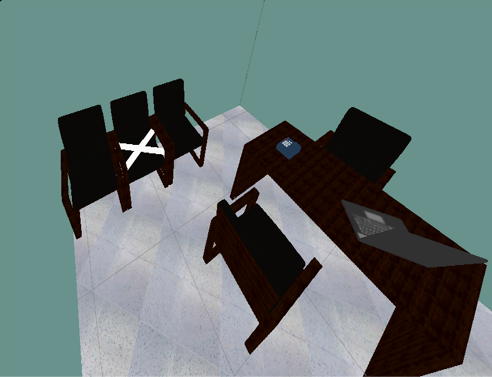
\includegraphics[width=\textwidth]{Metodologia/VE.png}
        \caption{Virtual environment screenshot}
        \label{fig:ve_photo}
    \end{subfigure}
    \hfill
    \begin{subfigure}[b]{0.49\textwidth}
        \centering
        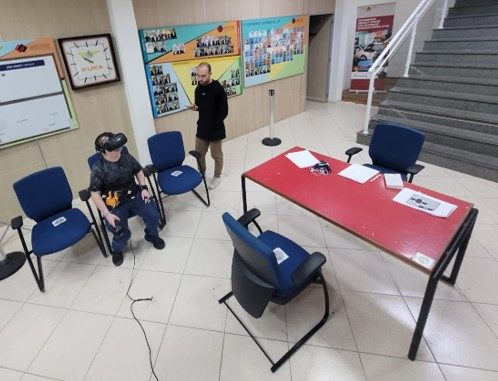
\includegraphics[width=\textwidth]{Metodologia/RE.jpg}
        \caption{Real environment photo}
        \label{fig:re_photo}
    \end{subfigure}
       \caption{Environment comparisson}
       \label{fig:ve_re}
\end{figure}